% Figure from MATH 591 notes, section 50. Compile with the notes preamble.
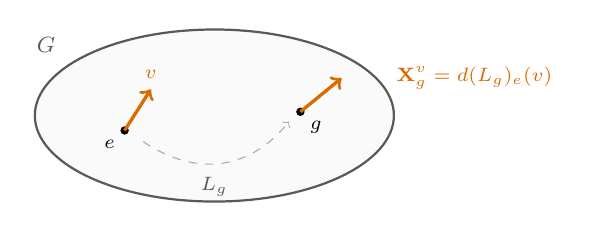
\begin{tikzpicture}[scale=0.95]
\draw[thick, gray!70!black, fill=gray!4] (0,0) ellipse (2.4 and 1.15);
\node[gray!70!black, font=\footnotesize] at (-2.25,0.95) {$G$};
\fill (-1.2,-0.2) circle (1.6pt) node[below left, font=\scriptsize] {$e$};
\fill (1.15,0.05) circle (1.6pt) node[below right, font=\scriptsize] {$g$};
\draw[->, very thick, orange!85!black] (-1.2,-0.2) -- ++(0.35,0.55) node[above, font=\scriptsize] {$v$};
\draw[->, very thick, orange!85!black] (1.15,0.05) -- ++(0.55,0.45) node[right, xshift=16pt, font=\scriptsize] {$\mathbf{X}^v_g = d(L_g)_e(v)$};
\draw[->, dashed, gray!65] (-0.95,-0.35) .. controls (-0.2,-0.85) and (0.5,-0.7) .. (1.0,-0.08);
\node[gray!70!black, font=\scriptsize] at (0.0,-0.95) {$L_g$};
\end{tikzpicture}
